\section{Objects} \label{sec:Objects}

When processing the CMS data and simulated physics samples described in Section \ref{sec:samples}, a particle flow (PF) \cite{CMS:2017yfk} algorithm is used in order to define objects from real or simulated CMS detector information. Objects corresponding to the following particles are utilized in the analysis: Photons, electrons, muons, and ``jets'' resulting from hadronized quarks or gluons. In addition, a special object called ``MET'' (Missing transverse momentum) is utilized in order to tag events which may contain particles which evade detection such as neutrinos. 

The same object definitions are used for all WW$\gamma\gamma$ final state categories when reconstructing objects from both data and simulation events.

In this section, the choice and reconstruction of the following objects is described: Vertex choice in Section \ref{sec:vertex}, photons in Section \ref{sec:photons}, electron and muons in Section \ref{sec:LeptonSelections}, jets in Section \ref{sec:Jets} and MET in Section \ref{sec:MET}. Finally, the yields and efficiencies of the signal and background processes in this analysis after the selections described in this section are described in Section \ref{sec:Preselection_yields}.

\subsection{Vertex} \label{sec:vertex}

Because there can be many simultaneous interactions in a given CMS event due to the large number of protons in colliding LHC protons bunches, many interactions points may be reconstructed. In order to identify the vertex corresponding to the highest energy interaction of the proton-proton collisions, called the ``hard interaction'', the vertex which has the highest sum of $p_{T}^{2}$ is chosen as the point from which photons are reconstructed and from which jets are taken. This is chosen as in the WW$\gamma\gamma$ processes, high $p_{T}$ tracks from the WW decay products are expected, namely from leptons and jets.

In Figure \ref{fig:VtxEff}, the probability of choosing a vertex with a z-position along the colliding axis within $|dZ|$ of the z-position of the generator level vertex is shown for the 2017 SM at NLO semi-leptonic signal sample. It is shown from the first few points
that the selected reconstructed vertex has an absolute z position within 0.1cm of the z position of the generator vertex for more than 99\% of events. This indicates that the choice of the vertex with the highest sum of $p_{T}^{2}$ is an appropriate choice for the HH$\rightarrow$WW$\gamma\gamma$ process. 

\begin{figure}[H]
    \centering
    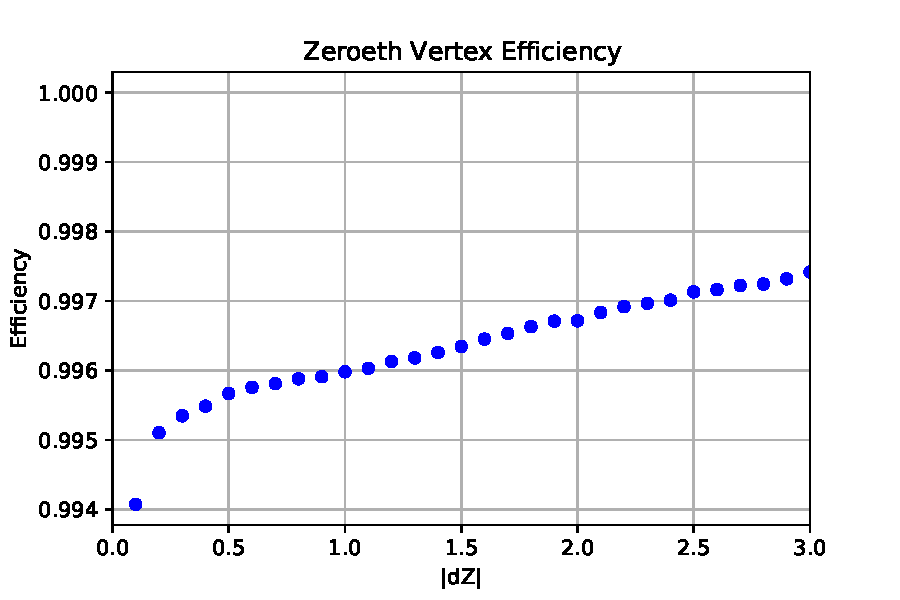
\includegraphics[width=0.75\textwidth]{Sections/HHWWgg/images/Objects/VtxEff.pdf}
    \caption{Efficiency vs $|dZ|$ for the Semi-Leptonic Signal}
\label{fig:VtxEff}
\end{figure}

\subsection{Photons} \label{sec:photons}

Photons used in this analysis are selected from the PF set of photon candidates.
The energy of each photon candidate is estimated from the Supercluster (SC), which
includes deposits from the many particles comprising the electromagnetic shower. In
some cases, photons will interact with detector material upstream of the ECAL and
produce an electron-positron pair; these are known as ``converted'' photons. Converted
photons will also deposit energy in the ECAL preshower detector (ES), which is included
in the SC energy estimate. A correction is then made to this SC energy using a
multivariate regression technique~\cite{Sirunyan:2018ouh}. After that, data and MC are brought into agreement
by applying additional scale and smearing corrections to the photon energies. Once the
photon energy has been established, a set of preselection criteria is applied to obtain the
final set of photons considered in the analysis. One of these criteria is a requirement
placed on the output score of the photon identification BDT, which is trained to
reduce the contamination from other objects which mimic real photons. 

All data events are required to have fired the high-level trigger (HLT) double photon paths and pass diphoton preselections. Simulated events are only required to pass diphoton preselections, defined to be tighter than the HLT dataset requirements. 

The HLT trigger paths used in this analysis are defined in Section \ref{sec:data_samples}, and require the presence of two isolated photons with one photon \pt higher than 30 GeV and the other one with a \pt of at least 18 GeV for 2016 or 22 GeV for 2017 and 2018 in order to keep the bandwidth of the HLT at sustainable levels. The trigger efficiency of each year is measured using data collected at the LHC by CMS and is applied to simulation samples. Higgs candidates with diphoton decays are then built from pairs of photon candidates.

Photon candidates are subject to a pre-selection that imposes requirements on photon kinematics, hadronic leakage, and shower shape. The pre-selection is designed to be slightly more stringent than the trigger requirements, where the pre-selection cuts are summarized in Table~\ref{tab:preselection}. 
The shower shape and isolation variables in simulation are corrected with
a chained quantile regression method~\cite{DBLP:journals/corr/abs-1211-6581}
based on studies of \Ztoee events.
Each variable is corrected with a separately trained boosted decision tree (BDT),
taking the photon kinematic properties, per-event energy density, and the previously corrected features as inputs to ensure that correlations between the inputs are preserved and closer to those in data.
This correction method also improves the modeling of the photon identification (photon ID)
discriminant in MC simulation with respect to the previous CMS~\Htogg results~\cite{Sirunyan:2018ouh}.
A multivariate identification method, based on photon shower-shape, isoaltion and kinematic variables, is used to separate \Htogg signal from background photons (photon ID). A very loose requirement on the photon ID score above -0.9 is applied as a further selection, which eliminates a very significant amount of non-prompt photons while keeping almost 100$\%$ of prompt photons.
Each photon candidate is required to satisfy the ``conversion-safe" electron-veto, which aims to reject photon objects which may have been reconstructed from real electrons.

Additionally, both photons must pass either \RNINE$>$ 0.8,
 $Iso_{ch,had}<$ 20 GeV, or $Iso_{ch,had}$/ \pt $<$ 0.3 if their \pt is above 14 GeV and H/E is below 0.15. \RNINE is defined as the energy sum of the 3 × 3 crystal matrix centered on the most energetic
crystal in a given ECAL supercluster, divided by the energy of the supercluster, and H / E represents the ratio of hadronic energy to electromagnetic energy.

\begin{table}[htbp]
        \caption{List of photon preselection requirements.}
        \begin{center}
                \begin{tabular}{|l|l|l|l|l|l|}
                        \hline
                        & H/E     & $\sigma_{i\eta i\eta}$ & \RNINE & $Iso_{ph}$ & $Iso_{track}$ \\
                        \hline
                        EB; R9$>$  0.85   & $<$0.08 & --       & $>$0.5  & -- & --\\
                        \hline
                        EB; R9$\leq$0.85  & $<$0.08 & $<$0.015 & $>$0.5  & $<4.0$ & $<6.0$\\
                        \hline
                        EE; R9$>$0.90     & $<$0.08 & --       & $>$0.8  & -- & --\\
                        \hline
                        EE; R9$\leq$0.90  & $<$0.08 & $<$0.035 & $>$0.8  & $<4.0$ & $<6.0$\\
                        \hline
                \end{tabular}
        \end{center}
        \label{tab:preselection}
\end{table}

Preselection efficiencies and the loose photon ID cut efficiency are determined from data using \Ztoee~ events with the tag and probe method. By definition the tag and probe technique using \Ztoee~ does not allow for the measurement of the electron-veto efficiency, which instead is measured independently using \Ztommg~ events. The scale factors, defined as the ratio of efficiency in data to efficiency in simulation, are used to correct the signal efficiency in simulated signal samples and the uncertainties are propagated to the expected signal yields.

Each event is required to have at least one diphoton candidate constructed with respect to the
zeroth vertex that passes the preselections described above. The largest-\pt photon (leading) is required to have
\pt $>$ 35 GeV and the second largest (subleading) is required to
have  \pt $>$ 25 GeV. These photons must also pass a loose selection on a dedicated $H\rightarrow\gamma\gamma$ photon ID shown in Table \ref{tab:PhotonSelections}.

\begin{table}[htbp]
        \begin{center}
                \begin{tabular}{c|cc}
                         \hline
                         & Leading Photon & Subleading Photon \\ \hline
                         %$\frac{p_{T}}{m_{\gamma\gamma}}$ & (1/3) & (1/4) \\
                         Photon ID & -0.9 & -0.9 \\ \hline
                \end{tabular}
        \end{center}
        \caption{Additional photon object selections}
        \label{tab:PhotonSelections}
\end{table}


Finally, the events with the invariant mass of two photons within $100 < \mgg < 180$ GeV, are selected for the signal extraction.

\subsection{Leptons} \label{sec:LeptonSelections}

In this analysis, electron and muon objects are considered, and the analysis remains agnostic to tau leptons, as they are neither tagged nor rejected. Because the number of leptons is used as a handle of orthogonality between the three final state categories, it is necessary that all final state categories apply the same lepton selections. A possible way to improve this analysis in the future would be to include the tagging of tau leptons, which may be present in the leptonic WW$\gamma\gamma$ final states. 

For electrons and muons, ID MVA outputs are utilized in order to identify leptons with different balances of sensitivity and yields. Additionally, isolation criteria is defined and utilized in order to quantify how isolated leptons are from other objects. The decision of which electron ID, muon ID and muon isolation to select comes from comparing the ratio of signal yields after preselections and subsequent lepton selections for the two final state categories containing leptons: the semi-leptonic and fully-leptonic final states. This figure is checked
when applying a loose cut based electron ID with a tight Muon ID and isolation, versus applying a medium MVA based electron ID with a medium Muon ID and isolation. Comparing the ratios between sets of lepton
selections allows one to observe which categories lose the most signal due to the corresponding lepton selections. The relative yields are shown in Table \ref{tab:LeptonSelectionYields}.

\begin{table}[htbp]
    \begin{center}
            \begin{tabular}{|c|c|c|c|c|c|c|}
                    \hline
                    Category & $SL_{e}$ & $SL_{\mu} $ & $FL_{ee}$ & $FL_{\mu\mu}$ & $FL_{e\mu}$ & $FL_{\mu e}$ \\
                    \hline
                    Loose Electron, Tight Muon   & 0.16 & 0.20 & 0.018  & 0.053 & 0.038 & 0.037  \\
                    \hline
                    Medium Electron, Medium Muon  & 0.023 & 0.228 & 0.0006  & 0.062 & 0.0067 & 0.005 \\
                    \hline
                    Ratio & 0.14375 & 1.14 & 0.0333 & 1.17 & 0.176 & 0.135 \\
                    \hline
            \end{tabular}
    \end{center}
    \caption{Ratio of signal yields after preselections and \pt/\mgg cuts over the addition of lepton requirements, and the ratio between the two pairs of lepton requirements. In this analysis, the selections in the top row are used (Loose electron, tight muon), while the other two rows are produced in order to determine the ideal combination of lepton selections to use. \label{tab:LeptonSelectionYields}}
\end{table}

In the Fully-Hadronic final state category, events are required to contain exactly zero leptons. This means that the choice of lepton selection can impact the FH yields, as it may change whether an event has zero leptons or not. The ratio of FH signal yield between the two sets of lepton IDs and ISOs is found to be
0.947, where about 5\% of signal events are lost when using medium MVA based electron ID and medium Muon ID and ISO.

Exactly one lepton is required to pass selections in the SL (Semi-Leptonic) category, therefore for this check the yields for this process are split into the $SL_{e}$ (Semi-Leptonic electron) and $SL_{\mu}$ (Semi-Leptonic muon)
subcategories. For the FL (Fully-Leptonic) category, it is required that exactly two leptons pass the common set of lepton selections, and therefore for the purpose of this check, this process is split into four sub-categories corresponding to the flavours of the
leading two leptons. 

Applying a medium MVA based electron ID reduced subcategory yields containing electrons by factors of 0.14375, 0.0333, 0.176 and 0.135, while subcategories containing a muon
change by factors of 1.14, 1.17, 0.176 and 0.135. While a slight gain is obtained from loosing the muon ID and isolation, most signal events are rejected from tightening electron ID, especially
in the di-electron FL subcategory whose ratio of selected events to pre-selected events is reduced by a factor of about 30.

Because a DNN method is applied in the Semi-Leptonic final state, it is desirable to use looser selections in order to keep more events to input for training. In the Fully-Leptonic analysis,
as the expected yield is already low, it is desirable to preserve signal while also maintaining enough events in the data sideband regions to perform a data driven background fit. For muon subcategories,
as the yields are not affected drastically by tightening the muon ID and isolation from medium to tight, these selections are determined desirable in order to tag muons with
greater purity.

Therefore, all electrons are required to pass a loose cut based ID, and muons are required to pass a Tight ID and posses a relative PF isolation value in a cone of $\Delta R < 0.4$ less than 0.15, as defined in Eq. \ref{eqn:MuonIsoDef}. This is
required for all three final state categories.

\subsubsection{Electrons}

% https://github.com/cms-analysis/flashgg/blob/4e958a7c7997466be6c95115734527577d9d88d8/MicroAOD/python/flashggLeptonSelectors_cff.py
All PF Electrons considered must pass a group of selections in order to consistitue a high $p_{T}$ electron that may have come from a leptonically decaying W boson.
Each electron is required to pass the selections in Table \ref{tab:ElectronSelections}. Scale factors corresponding to loose cut based electron ID are applied as a multiplicative factor to
the central event weight to account for the discrepancy in data / MC electron ID assignment. 

In addition to a loose electron ID, electron candidates are required to have $p_{T} > $ 10 GeV, and a pseudorapidity in the range (0 $<$ $|\eta|$ $<$ 1.4442) or (1.566 $<$ $|\eta|$ $<$ 2.5) in order to remain in the CMS tracker region and avoid the ECAL overlap region. Furthermore, a distance parameter value ($\Delta R = \sqrt{(\Delta\eta)^{2} + (\Delta\phi)^{2}}$) greater than 
0.4 is required between each electron candidate and each of the two photon candidates from the event's highest $p_{T}$ diphoton in order to select isolated electron candidates. A distance parameter value 
of less than 0.4 is also required between the electron candidate's track and ECAL supercluster position, and a 
distance parameter value with each jet candidate $>$ 0.4 is required. Finally, the invariant mass of the electron with each photon candidate in the event's highest \pt diphoton 
candidate must be at least 5 GeV greater or less than the Z boson mass in order to avoid selecting events coming from Z$\rightarrow$ee decays. 

\begin{table}[H]
    \begin{center}
        \begin{tabular}{c|c}
        Variable & Selection \\ \hline
        $p_{T}$ [GeV] & $>$ 10 \\
        $|\eta|$ & (0 $<$ $|\eta|$ $<$ 1.4442) or (1.566 $<$ $|\eta|$ $<$ 2.5) \\
        ID & Loose Cut Based \\
        $\Delta R(e^{-},\gamma)$ & $>$ 0.4 \\
        $\Delta R(e^{-},jet)$ & $>$ 0.4 \\
        $\Delta R(track_{e^{-}},SC_{e^{-}})$ & $<$ 0.4 \\
        $|m_{e^{-}\gamma}$ - 91.187$|$ [GeV] & $>$ 5
        \end{tabular}
    \end{center}
    \caption{
        Electron object requirements
    }
    \label{tab:ElectronSelections}
\end{table}

\subsubsection{Muons}

Selections are applied to all muon objects with the aim of identifying a muon coming from a leptonically decaying W boson. Each muon object is required to pass
the selections in Table \ref{tab:MuonSelections}. In addition to a tight Muon ID, muon candidates are required to have $p_{T} > $ 10 GeV, a pseudorapidity in the range ($|\eta| < 2.4$) to remain in the CMS tracker region, a distance parameter value with each photon candidate $>$ 0.4, a 
distance parameter value with each jet candidate $>$ 0.4, and an isolation $<$ 0.15, as defined in Eq. \ref{eqn:MuonIsoDef}, in order to select isolated muon candidates, where sumPUPt is the summed transverse momentum of charged particles not from the primary vertex.

\begin{table}[H]
    \begin{center}
        \begin{tabular}{c|c}
        Variable & Selection \\ \hline
        $p_{T}$ [GeV] & $>$ 10 \\
        $|\eta|$ & $<$ 2.4 \\
        ID & Tight \\
        $\Delta R(\mu,\gamma)$ & $>$ 0.4 \\
        $\Delta R(\mu,jet)$ & $>$ 0.4 \\
        $I_{\mu}$ & $<$ 0.15
        \end{tabular}
    \end{center}
    \caption{
        Muon object requirements
    }
    \label{tab:MuonSelections}
\end{table}

Scale factors for each year corresponding to the applied tight muon ID are applied to the event weight for each lepton passing all Muon selections, in order to improve the agreement between data and simulation.

\begin{equation}
   I_{\mu} = \frac{( sumChargedHadronPt + max(0, sumNeutralHadronEt + sumPhotonEt - \frac{sumPUPt}{2}) )}{p^{\mu}_{T}}
   \label{eqn:MuonIsoDef}
\end{equation}
% https://twiki.cern.ch/twiki/bin/view/CMSPublic/SWGuideMuonId %% Muon ID definition
\subsection{Jets} \label{sec:Jets}

Jets are constructed using the anti-$k_{T}$ clustering method with a distance parameter of 0.4, classifying them as ``AK4 jets". The selections applied on jets are
shown in Table \ref{tab:JetSelections}. Jet candidates are 
required to have $p_{T} > $ 25 GeV, an absolute value of pseudorapidity $<$ 2.4, are required to pass a loose PU Jet ID in order to avoid reconstructing
jets from pileup interactions, a distance parameter value $>$ 0.4 between the jet 
candidate and each photon candidate from the diphoton candidate, and a distance parameter $>$ 0.4 with any electron and muon candidates which pass the previously defined 
electron and muon selections. Jet corrections applied include jet energy corrections and a jet energy regression.

\begin{table}[H]
    \begin{center}
        \begin{tabular}{c|c}
        Variable & Selection \\ \hline
        $p_{T}$ [GeV] & $>$ 25 \\
        $|\eta|$ & $<$ 2.4 \\
        ID & Tight \\
        PU Jet ID & Loose \\
        $\Delta R(j,\gamma_{l})$ & $>$ 0.4 \\
        $\Delta R(j,\gamma_{sl})$ & $>$ 0.4 \\
        $\Delta R(j,e^{-})$ & $>$ 0.4 \\
        $\Delta R(j,\mu)$ & $>$ 0.4 \\

        \end{tabular}
    \end{center}
    \caption{
        Jet requirements
    }
    \label{tab:JetSelections}
\end{table}

In addition, jets from the hadronization of bottom quarks are tagged using a Deep Neural Network (DNN) that takes secondary vertices and PF 
candidates as inputs \cite{Sirunyan:2017ezt}. The output of this DNN is referred to as the b-tagging score. In the Semi-Leptonic and Fully-Hadronic categories, the b-tagging score is input as a training variable
in Deep Neural Network trainings, and therefore no selection is applied before training. In the Fully-Leptonic category, medium b-tagging working points
for the years 2016, 2017 and 2018 are applied to all jets. This decision is based on the event yields of the 2017 HH SM NLO signals, and of the associated production of H$\rightarrow\gamma\gamma$ with a pair of top quarks process (ttH), a prominent b-quark background
in the WW$\gamma\gamma$ phase space due to b-quarks coming from the t$\rightarrow$bW decay. 

For each event, an event is considered b-vetoed if it contains at least one jet with a b-tagging score greater than a given threshold. The value of this threshold was scanned from 0 to 1, using the b-tagging score, and the ratio of process yields with and without a b-veto applied are shown for the WW$\gamma\gamma$ signal and
the ttH background process in Figure \ref{fig:YieldVsBThresh}, and a ratio of the two is shown in Figure \ref{fig:SigttHRatiovsbThresh}, where the three vertical lines represent
the Loose, Medium and Tight working points as defined by the CMS Jet-Met physics object group (POG).

\begin{figure}[H]
    \setcounter{subfigure}{0}
    \centering
    \subfloat[WW$\gamma\gamma$ Signal]{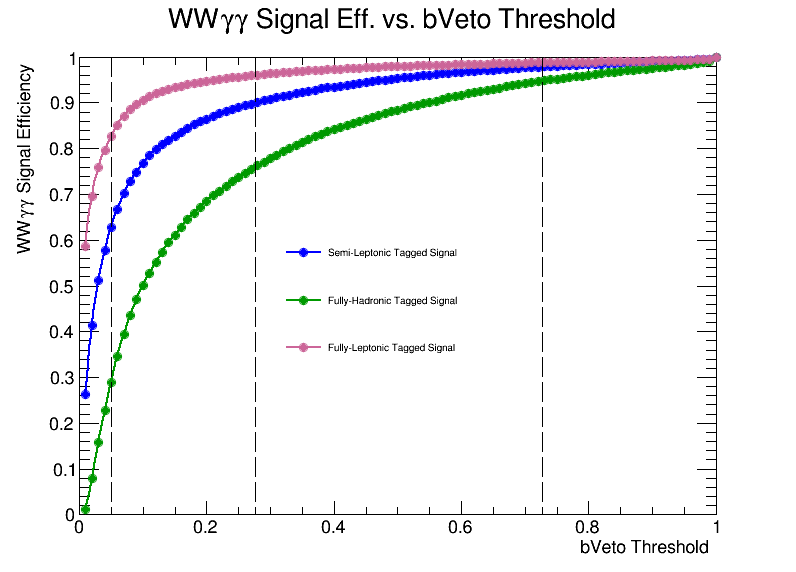
\includegraphics[width=0.45\textwidth]{Sections/HHWWgg/images/Objects/SigEffvsbVeto.png}}
    \qquad
    \subfloat[ttH]{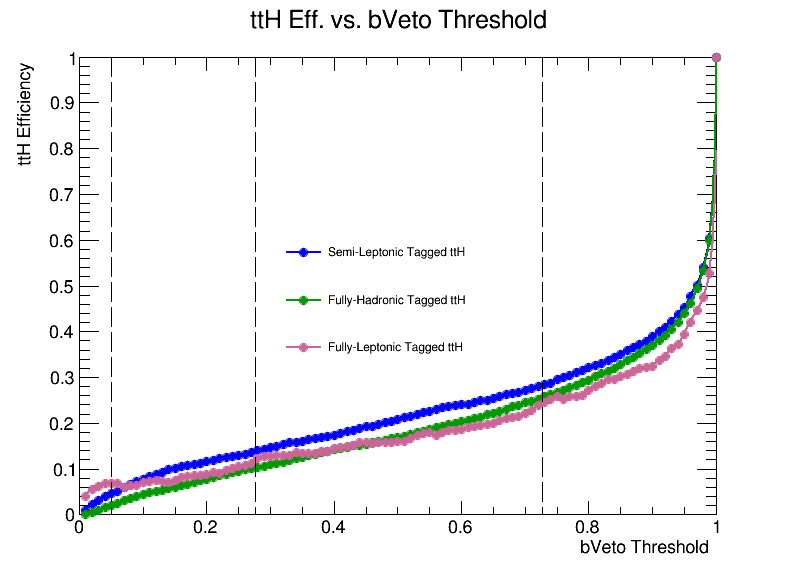
\includegraphics[width=0.45\textwidth]{Sections/HHWWgg/images/Objects/ttHvsbVeto.png}}
    \caption{2017 Signal and ttH background signal yields, relative to signal yield with no bVeto, vs. bVeto threshold}
    \label{fig:YieldVsBThresh}
\end{figure}

\begin{figure}[H]
    \centering
    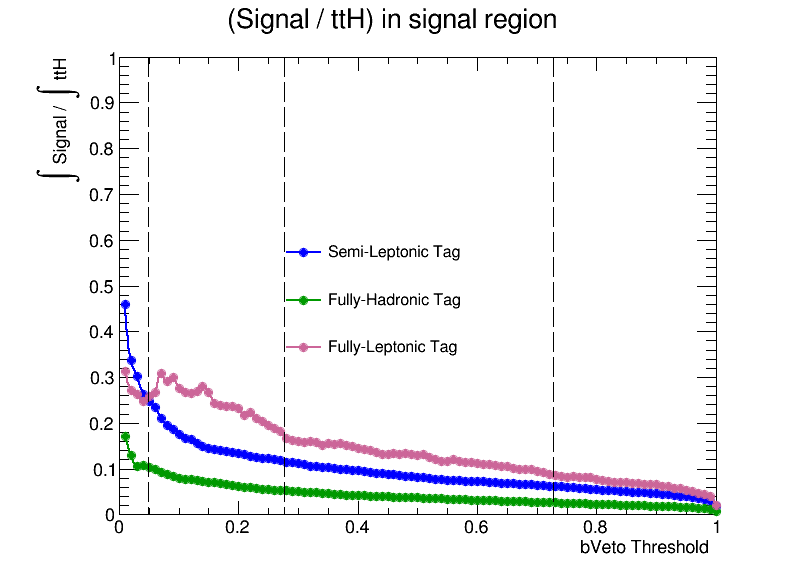
\includegraphics[width=0.75\textwidth]{Sections/HHWWgg/images/Objects/sigttHRatiovsbveto.png}
    \caption{Ratio of ttH signal region events over WW$\gamma\gamma$ signal events in signal region vs. bVeto threshold}
\label{fig:SigttHRatiovsbThresh}
\end{figure}

The signal efficiency curves look as expected for the three final states: The Fully-Leptonic final state is overall the most efficient because there are no quarks in its signal, Semi-Leptonic comes next
as it contains two quarks in its signal, and the Fully-Hadronic signal is the least efficient overall as it contains four quarks in its signal, and therefore is the most likely
to contain a jet with a higher b score due to high values of important b-tagging variables such as $p_{T}$. The ttH signal events as categorized by the three WW$\gamma\gamma$ categories have similar efficiencies among the three
categories, with about 75\% of events rejected from vetoing an event with at least one tightly b-tagged jet.

For the Semi-Leptonic and Fully-Hadronic final state categories, no b-veto is applied but rather is used as an input variable into DNN trainings. In order to properly reshape the MC b-tagging score distribution,
a btag-reshape scale factor is applied to these event weights for each jet passing event selections.

For the Fully-Leptonic final state category, the medium b-tagging score working point is applied as only about 5\% of signal is rejected, while about 85\% of ttH background is rejected.
Events falling into the fully-leptonic category are vetoed if they contain at least one jet with a b-tagging score greater than the medium working point.

The decision to apply a loose PU Jet ID to all jets with $p_{T}$ below 50 GeV comes from comparing the Fully-Hadronic final state category signal and data yields in the data sideband (defined as [100 $<$ $\mgg$ $<$ 115] or [135 $<$ $\mgg$ $<$ 180 GeV]) when applying
different PU Jet IDs. This category requires at least four jets, so applying different PU Jet ID requirements on all jets results in different yields, as shown in Figure \ref{fig:PUJetID},
with yields summarized in Table \ref{tab:PUJetIDYields}.

\begin{figure}[H]
    \setcounter{subfigure}{0}
    \centering
    \subfloat[Data Sidebands]{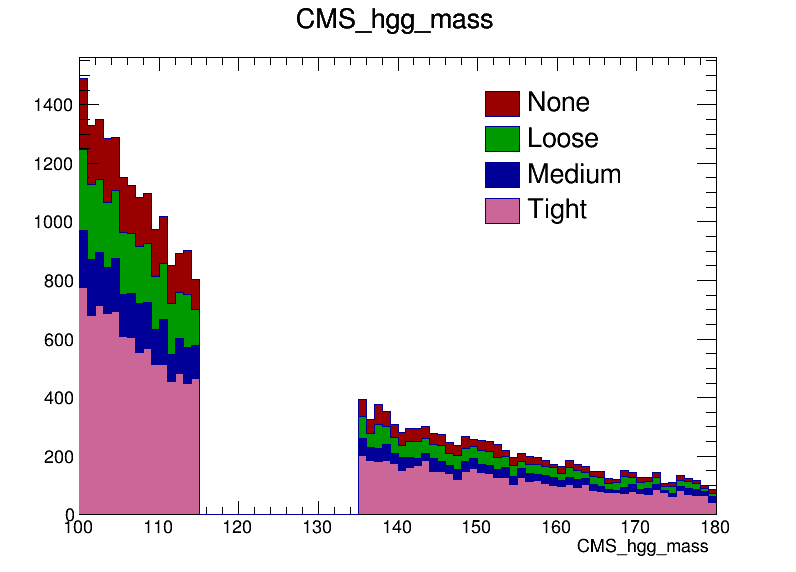
\includegraphics[width=0.45\textwidth]{Sections/HHWWgg/images/Objects/PUJet_ID_Sidebands.png}}
    \qquad
    \subfloat[Signal Region]{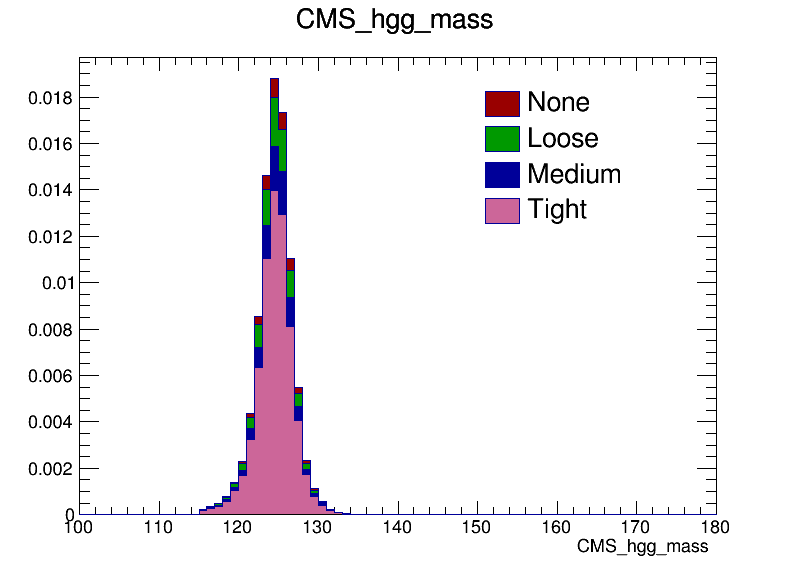
\includegraphics[width=0.45\textwidth]{Sections/HHWWgg/images/Objects/PUJet_ID_SR.png}}
    \caption{2017 Data (Signal) diphoton mass distributions in the sideband (signal) region for the Fully-Hadronic tagged category.}
    \label{fig:PUJetID}
\end{figure}

\begin{table}[!htbp]
    \begin{center}
            \begin{tabular}{|c|c|c|c|c||c|}
                    \hline
                    PUJet ID & Data Sidebands & Signal Region & Data Ratio to None & Signal Ratio to None & $\frac{S}{\sqrt{B}}$\\
                    \hline
                    None & 25940 & 0.09015 & 1 & 1 & 1 \\
                    \hline
                    Loose & 22119 & 0.08625 & 0.853 & 0.957 & 1.036 \\
                    \hline
                    Medium & 17418 & 0.07644 & 0.672 & 0.848 & 1.035\\
                    \hline
                    Tight & 14001 & 0.06707 & 0.540 & 0.744 & 1.012\\
                    \hline
            \end{tabular}
    \end{center}
    \caption{Number of data events in data sidebands and 2017 SM NLO Fully-Hadronic events in signal region, and relevant ratios. \label{tab:PUJetIDYields}}
\end{table}

If it is assumed that the relative change in dataside band events is roughly proportional to the relative change of data events in the signal region (defined as 115 $<$ $\mgg$ $<$ 135 GeV), an estimated signal region $\frac{S}{\sqrt{B}}$
can be computed and is found to be maximized in the case of applying a Loose PU Jet ID. A similar value is obtained when applying Medium PUJetID, but considering they are within
0.1\% of each other at the trade-off of a loss of about 10\% of signal, it is optimal to apply a loose PU Jet ID for the Fully-Hadronic final state. As the Semi-Leptonic and Fully-Leptonic
final state categories do not explicitly select on jet number, and the loose PU Jet ID has a high efficiency and should therefore not affect the Semi-Leptonic and Fully-Leptonic
final states noticeably, all jets are required to pass the Loose PU Jet ID.

\subsection{MET} \label{sec:MET}

The missing transverse momentum vector \ptvecmiss (sometimes referred to as ``MET") is defined as the projection onto the plane perpendicular to the beam axis of the negative vector sum of the momenta of all reconstructed PF objects in an event. Its magnitude is referred to as \ensuremath{\pt^\text{miss}}\xspace. This variable is of importance when identifying events which may contain a neutrino coming from a leptonic W decay, as neutrinos escape the CMS detector undetected.

In the Semi-Leptonic final state, MET is used as an input variable in the DNN training. In the Fully-Hadronic final state, MET is not used. In the Fully-Leptonic final state, a selection of 20 GeV is required for MET.
Corrections applied include an XY correction and MET filters, where the MET filters applied to Data and MC for all three years are shown in Table \ref{tab:METfilters} in order to remove events which are flagged as bad due to various reasons including large HCAL noise, dead ECAL channels. For Data there is one additional MET filter applied: {\tt Flag\_eeBadScFilter}, corresponding to events tagged as having poor ECAL endcap super clusters. 

\begin{table}[H]
    \begin{center}
        \begin{tabular}{c}
        MET Filters \\ \hline
        {\tt Flag\_goodVertices} \\
        {\tt Flag\_globalSuperTightHalo2016Filter} \\
        {\tt Flag\_HBHENoiseFilter} \\
        {\tt Flag\_HBHENoiseIsoFilter} \\
        {\tt Flag\_EcalDeadCellTriggerPrimitiveFilter} \\
        {\tt Flag\_BadPFMuonFilter} \\ 
        \end{tabular}
    \end{center}
    \caption{
        MET filters applied to Data and MC for all three years of data taking and detector conditions. 
    }
    \label{tab:METfilters}
\end{table}

\subsection{Preselection yields} \label{sec:Preselection_yields}

In this section, the yields and efficiencies of each 2017 signal and background MC process described in Section \ref{sec:samples} are shown before and after all object selections and final state preselections are applied in order to understand the major background processes to be targeted in each final state's subsequent selections. 

Preselections are defined as the common object and event selections described in the above subsections, in addition to the orthogonality selection applied for each final state: 
Events in the Semi-leptonic category are required to have exactly one lepton passing the common lepton selections, events in the Fully-hadronic category are required to have at least four jets and exactly 
zero leptons passing the common jet and lepton selections, and events in the Fully-leptonic category are required to have exactly 2 leptons passing the common lepton selections. 

The yields and process efficiencies before and after each final state's pre-selections are shown in Tables \ref{tab:Continuum_Background_Yield_Table}, \ref{tab:Single_Higgs_Yield_Table} and \ref{tab:HH_Yield_Table} below. Additionally,
the individual contribution of each MC sample with respect to the total MC yield for a given set of selections (Before preselection, Semi-leptonic preselections, Fully-hadronic preselections or Fully-Leptonic preselections)
are shown in Tables \ref{tab:Continuum_Background_Contribution_Table} and \ref{tab:Single_Higgs_Contribution_Table}. Note that processes with an absolute number of simulated events less than 1000 (less than 100 in the fully-leptonic final category) are given a null value or only an efficiency is reported, as their low number of events implies that their corresponding processes would have a poor simulated description and potentially a large statistical uncertainty. 

\begin{figure}[H]
        \resizebox{1\textwidth}{!}{%
                \begin{tabular}{c|c|c|c|c}
                        MC Sample & Before preselection & SL (efficiency) & FH (efficiency) & FL (efficiency) \\ \hline
                         %DiPhotonJetsBox\_M40\_80 & 1138.8964 & - (-\%) & - (-\%) & - (-\%) \\
                         $\gamma\gamma+$jets & 302977.6194 & 542.4641 (0.179\%) & 6246.9949 (2.062\%) & 2.7749 (0.001\%) \\
                        %  DYJetsToLL\_M-50 & 7525.2616 & - (-\%) & - (-\%) & - (-\%) \\
                         THQ\_ctcvcp & 3.4592 & 0.5789 (16.735\%) & 1.0579 (30.582\%) & 0.0012 (0.034\%) \\
                         TTGG\_0Jets & 44.0507 & 10.9847 (24.936\%) & 25.6024 (58.12\%) & 0.1487 (0.338\%) \\
                         TTGJets\_TuneCP5 & 765.4892 & 154.6684 (20.205\%) & 402.1377 (52.533\%) & ($<$0.2\%) \\
                        %  TTToHadronic & 903.4816 & - (-\%) & - (-\%) & - (-\%) \\
                         ttWJets & 5.0469 & ($\approx$21\%) & 2.8337 (56.147\%) & ($<$0.1\%) \\
                        %  W3JetsToLNu & 1041.188 & - (-\%) & - (-\%) & - (-\%) \\
                        %  W4JetsToLNu & 985.8018 & - (-\%) & - (-\%) & - (-\%) \\
                        %  WGGJets & 534.8559 & - (-\%) & - (-\%) & - (-\%) \\
                        %  WGJJToLNu\_EWK\_QCD & 367.5752 & - (-\%) & - (-\%) & - (-\%) \\
                        %  WGJJToLNuGJJ\_EWK & 65.3279 & - (-\%) & - (-\%) & - (-\%) \\
                        %  WWTo1L1Nu2Q & 337.0574 & - (-\%) & - (-\%) & - (-\%) \\
                        %  WW\_TuneCP5 & 189.1288 & - (-\%) & - (-\%) & - (-\%) \\
                         GJet & 830909.3171 & 1061.0649 (0.002\%) & 2466.3582 (0.002\%) & ($<$0.001\%) \\
                         QCD & 1653618.4935 & ($<$0.001\%) & ($<$0.001\%) & ($<$0.001\%) \\
                         TTJets & 23.5628 & 3.3477 (81.397\%) & 18.8106 (55.121\%) & ($<$2\%) \\
                         W1Jet & 5838.2419 & 245.2825 (0.329\%) & ($<$0.5\%) & ($<$0.5\%) \\
                         W2Jets & 5589.4864 & 352.6322 (0.343\%) & 204.2186 (0.232\%) & ($<$0.5\%) \\ \hline
                         Total & 2812863.3417 & 2371.0234 (0.0008\%) & 9368.014 (0.0033\%) & 2.9248 (0.0\%) \\ \hline
                \end{tabular}}
        \captionof{table}{2017 Continuum Background MC before and after preselections for each final state, and process efficiency. Note that for processes with less than 1000 unweighted MC events after a selection (100 for the fully-leptonic preselections), a null value or only efficiency is shown.}
        \label{tab:Continuum_Background_Yield_Table}
\end{figure}

\newpage 

\begin{figure}[H]
        \resizebox{1\textwidth}{!}{%
                \begin{tabular}{c|c|c|c|c}
                        MC Sample & Before preselection & SL & FH & FL \\ \hline
                         %DiPhotonJetsBox\_M40\_80 & 0.0405\% & -\% & -\% & -\% \\
                         $\gamma\gamma+$jets & 10.7711\% & 22.8789\% & 66.6843\% & 94.8755\% \\
                        %  DYJetsToLL\_M-50 & 0.2675\% & -\% & -\% & -\% \\
                         THQ\_ctcvcp & 0.0001\% & 0.0244\% & 0.0113\% & 0.0397\% \\
                         TTGG\_0Jets & 0.0016\% & 0.4633\% & 0.2733\% & 5.0849\% \\
                         TTGJets\_TuneCP5 & 0.0272\% & 6.5233\% & 4.2927\% & -\% \\
                        %  TTToHadronic & 0.0321\% & -\% & -\% & -\% \\
                         ttWJets & 0.0002\% & -\% & 0.0302\% & -\% \\
                        %  W3JetsToLNu & 0.037\% & -\% & -\% & -\% \\
                        %  W4JetsToLNu & 0.035\% & -\% & -\% & -\% \\
                        %  WGGJets & 0.019\% & -\% & -\% & -\% \\
                        %  WGJJToLNu\_EWK\_QCD & 0.0131\% & -\% & -\% & -\% \\
                        %  WGJJToLNuGJJ\_EWK & 0.0023\% & -\% & -\% & -\% \\
                        %  WWTo1L1Nu2Q & 0.012\% & -\% & -\% & -\% \\
                        %  WW\_TuneCP5 & 0.0067\% & -\% & -\% & -\% \\
                         GJet & 29.5396\% & 44.7513\% & 26.3274\% & -\% \\
                         QCD & 58.7877\% & -\% & -\% & -\% \\
                         TTJets & 0.0008\% & 0.1412\% & 0.2008\% & -\% \\
                         W1Jet & 0.2076\% & 10.345\% & -\% & -\% \\
                         W2Jets & 0.1987\% & 14.8726\% & 2.18\% & -\% \\ \hline
                         Total & 100\% & 100\% & 100\% & 100\% \\ \hline
                \end{tabular}}
        \captionof{table}{Contribution w.r.t total 2017 Continuum Background MC for various phase spaces: Before and after preselections for each final state. Note that for processes with less than 1000 unweighted MC events after a selection (100 for the fully-leptonic preselections), a null value is shown.}
        \label{tab:Continuum_Background_Contribution_Table}
\end{figure}

\newpage 

\begin{figure}[H]
        \resizebox{1\textwidth}{!}{%
                \begin{tabular}{c|c|c|c|c}
                        MC Sample & Before preselection & SL (efficiency) & FH (efficiency) & FL (efficiency) \\ \hline
                         GluGluHToGG & 2226.7151 & 2.5556 (0.115\%) & 18.3933 (0.826\%) & - (-\%) \\
                         ttHJetToGG & 23.8639 & 5.9022 (24.733\%) & 14.4288 (60.463\%) & 0.0545 (0.228\%) \\
                         VBFHToGG & 158.1456 & 0.3712 (0.235\%) & 1.0675 (0.675\%) & - (-\%) \\
                         VHToGG & 85.5536 & 10.0542 (11.752\%) & 4.4384 (5.188\%) & 0.0832 (0.097\%) \\ \hline
                         Total MC & 2494.2782 & 18.8832 (0.0076\%) & 38.328 (0.0154\%) & 0.1377 (0.0001\%) \\ \hline
                \end{tabular}}
        \captionof{table}{2017 Single Higgs MC before and after preselections for each final state, and process efficiency. Note that for processes with less than 100 unweighted MC events after a selection, a null value is shown.}
        \label{tab:Single_Higgs_Yield_Table}
\end{figure}

\begin{figure}[H]
        \resizebox{1\textwidth}{!}{%
                \begin{tabular}{c|c|c|c|c}
                        MC Sample & Before preselection & SL & FH & FL \\ \hline
                         GluGluHToGG & 89.3\% & 13.5\% & 48\% & -\% \\
                         ttHJetToGG & 0.96\% & 31.3\% & 37.6\% & 39.6\% \\
                         VBFHToGG & 6.34\% & 2.0\% & 2.8\% & -\% \\
                         VHToGG & 3.43\% & 53\% & 11.6\% & 60.4\% \\ \hline
                         Total & 100\% & 100\% & 100\% & 100\% \\ \hline
                \end{tabular}}
        \captionof{table}{Contribution w.r.t total 2017 Single Higgs MC for various phase spaces: Before and after preselections for each final state. Note that for processes with less than 1000 unweighted MC events after a selection (100 for the fully-leptonic preselections), a null value is shown.}
        \label{tab:Single_Higgs_Contribution_Table}
\end{figure}

\begin{figure}[H]
        \resizebox{1\textwidth}{!}{%
            \begin{tabular}{c|c|c|c|c}
                    MC Sample & Before preselection & SL (efficiency) & FH (efficiency) & FL (efficiency) \\ \hline
                     Semi-leptonic HH$\rightarrow WW\gamma\gamma$ & 0.3042 & 0.1044 (34.306\%) & - (-\%) & - (-\%) \\
                     Fully-hadronic HH$\rightarrow WW\gamma\gamma$ & 0.3012 & - (-\%) & 0.0966 (32.07\%) & - (-\%) \\
                     Fully-leptonic HH$\rightarrow WW\gamma\gamma$ & 0.0741 & - (-\%) & - (-\%) & 0.0098 (13.214\%) \\ \hline 
            \end{tabular}}
    \captionof{table}{2017 HH MC before and after preselections for each final state, and process efficiency. Note that for processes with less than 100 unweighted MC events after a selection, a null value is shown.} 
    \label{tab:HH_Yield_Table}
\end{figure}


The tables show that among the continuum background MC processes, the fully-leptonic final state has a very low absolute number of simulation events after pre-selections and requiring exactly two leptons passing the common lepton selections. This was a core reason for the decision to perform a cut-based analysis for this final state, as there are not nearly enough MC events in order to perform a reasonable MVA based analysis. In the fully-hadronic final state, where a large QCD multi-jet background is expected, there is a low absolute number of simulation events from QCD MC, prompting the use of a data-driven estimate of QCD. For all three final states, the non-resonant diphoton $+$ jets process acts as a major background. 

The single higgs resonant background tables indicate that, as expected, different single higgs processes have larger background contaminations among the different WW$\gamma\gamma$ final states due to their different process topologies. However, for all final states the ttH process has a relatively high efficiency due to the presence of two top quarks which decay into bbWW in the majority of cases. 

Finally, it is seen in the HH selection table that the semi-leptonic and fully-hadronic signal processes have similar signal efficiencies and yields after pre-selections. This may be due to their relatively high branching ratios compared to the FL final state. 